%%%%%%%%%%%%%%%%%%%%%%%%%%%%%%%%%%%%%%%%%
% Journal Article
% LaTeX Template
% Version 1.4 (15/5/16)
%
% This template has been downloaded from:
% http://www.LaTeXTemplates.com
%
% Original author:
% Frits Wenneker (http://www.howtotex.com) with extensive modifications by
% Vel (vel@LaTeXTemplates.com)
%
% License:
% CC BY-NC-SA 3.0 (http://creativecommons.org/licenses/by-nc-sa/3.0/)
%
%%%%%%%%%%%%%%%%%%%%%%%%%%%%%%%%%%%%%%%%%

%----------------------------------------------------------------------------------------
%	PACKAGES AND OTHER DOCUMENT CONFIGURATIONS
%----------------------------------------------------------------------------------------

\documentclass[twoside,twocolumn]{article}

\usepackage{blindtext} % Package to generate dummy text throughout this template 

\usepackage[sc]{mathpazo} % Use the Palatino font
\usepackage[T1]{fontenc} % Use 8-bit encoding that has 256 glyphs
\linespread{1.05} % Line spacing - Palatino needs more space between lines
\usepackage{microtype} % Slightly tweak font spacing for aesthetics

\usepackage[english]{babel} % Language hyphenation and typographical rules

\usepackage[hmarginratio=1:1,top=32mm,columnsep=20pt,left=2cm,right=2cm,top=2cm,bottom=2cm]{geometry} % Document margins
\usepackage[hang, small,labelfont=bf,up,textfont=it,up]{caption} % Custom captions under/above floats in tables or figures
\usepackage{booktabs} % Horizontal rules in tables

\usepackage{lettrine} % The lettrine is the first enlarged letter at the beginning of the text

\usepackage{enumitem} % Customized lists
\setlist[itemize]{noitemsep} % Make itemize lists more compact

\usepackage{abstract} % Allows abstract customization
\renewcommand{\abstractnamefont}{\normalfont\bfseries} % Set the "Abstract" text to bold
\renewcommand{\abstracttextfont}{\normalfont\small\itshape} % Set the abstract itself to small italic text

\usepackage{titlesec} % Allows customization of titles
\renewcommand\thesection{\Roman{section}} % Roman numerals for the sections
\renewcommand\thesubsection{\roman{subsection}} % roman numerals for subsections
\titleformat{\section}[block]{\large\scshape\centering}{\thesection.}{1em}{} % Change the look of the section titles
\titleformat{\subsection}[block]{\large}{\thesubsection.}{1em}{} % Change the look of the section titles

\usepackage{fancyhdr} % Headers and footers
\pagestyle{fancy} % All pages have headers and footers
\fancyhead{} % Blank out the default header
\fancyfoot{} % Blank out the default footer
\fancyhead[C]{Running title $\bullet$ May 2016 $\bullet$ Vol. XXI, No. 1} % Custom header text
\fancyfoot[RO,LE]{\thepage} % Custom footer text

\usepackage{titling} % Customizing the title section

\usepackage{hyperref} % For hyperlinks in the PDF

% Packages maison
\usepackage{amsmath,amssymb} % For including math equations, theorems, symbols, etc
\usepackage{mathtools}
\usepackage{bm}
\usepackage{graphicx} % Required for including images
\graphicspath{{../Figures/}} % Set the default folder for images
\usepackage{prettyref}

%----------------------------------------------------------------------------------------
%	TITLE SECTION
%----------------------------------------------------------------------------------------

\setlength{\droptitle}{-4\baselineskip} % Move the title up

\pretitle{\begin{center}\Huge\bfseries} % Article title formatting
\posttitle{\end{center}} % Article title closing formatting
\title{A database linking piano and orchestral MIDI scores for automatic projective orchestration \textbf{(RESTREINT LE CHAMP D'APPLICATION, C'EST DOMMAGE NON ?)}} % Article title
\author{%
\textsc{L\'eopold Crestel, Philippe Esling}\\[1ex] % Your name
\normalsize IRCAM \\ % Your institution
\normalsize \href{mailto:leopold.crestel@ircam.fr}{leopold.crestel@ircam.fr} % Your email address
%\and % Uncomment if 2 authors are required, duplicate these 4 lines if more
%\textsc{Jane Smith}\thanks{Corresponding author} \\[1ex] % Second author's name
%\normalsize University of Utah \\ % Second author's institution
%\normalsize \href{mailto:jane@smith.com}{jane@smith.com} % Second author's email address
}
\date{\today} % Leave empty to omit a date
\renewcommand{\maketitlehookd}{%
\begin{abstract}
\noindent This article introduces the Projective Orchestral Database \textbf{POD}, a freely-available collection of midi scores composed of pairs linking piano scores to their corresponding orchestrations. To our best knowledge, this is the first database of its kind. 
\textbf{This can allow to perform piano or orchestral prediction, but more importantly to try to learn the correlation between piano and orchestral scores.} (\textbf{TROP RESTRICTIF})
Hence, we introduce the projective orchestration task, which consists in learning to perform automatic orchestration of a piano score. 
This task can be seen as the generation of a symbolic time series (an orchestral score) conditioned by another symbolic time series (the piano score).
We show how this task can be addressed using learning methods and also provide methodological guidelines to use the database.
\end{abstract}
}

%----------------------------------------------------------------------------------------

\begin{document}

% Print the title
\maketitle

%----------------------------------------------------------------------------------------
%	ARTICLE CONTENTS
%----------------------------------------------------------------------------------------

\section{Introduction}
% Orchestration = definition
Orchestration is the subtle art of writing musical pieces for the orchestra by combining the properties of various instruments in order to achieve a particular musical idea. \cite{koechli_orch,Rimsky-Korsakov:1873aa}. 
% Orchestration projective
Among the variety of writing techniques for orchestration, we define as \textit{projective orchestration} \cite{esling2010dynamic} the technique which consists in first writing a piano score and then orchestrating it (akin to a projection orchestration, as depicted in \prettyref{fig:orch}). 
This technique has been used by classic composers for centuries. One such example is the orchestration by Maurice Ravel of \textit{Pictures at an exhibition}, a piano work written by Modest Mussorgsky.
% Dataset symbolic pour l'orchestration projective
This paper introduces the first symbolic dataset of projective orchestrations.
% Rapide description
It contains pairs of piano pieces and associated with their orchestration written by famous composers. For some pieces, several orchestrations can be found for one given piano score.
% Purpose
Hence, the purpose of this database is to offer a solid playground for studying the correlations involved in the transformation from a piano to an orchestral score.

The remainder of this paper is organized as follows. We detail the structure of the database (section II). Then,the automatic projective orchestration task is introduced (section III) along with an evaluation framework and several propositions of learning based models that rely on the database. Finally, we provide methodological guidelines and conclusions are provided in the last section.

\section{Dataset}
\subsection{A scientific investigation of orchestration}
% Teaching orchestration = exemples
\textbf{Over the past centuries,} several treatises have been written by notorious composers in an attempt to decipher some guiding rules in orchestration (\cite{koechli_orch,piston-orch,Rimsky-Korsakov:1873aa}).
Even though they compound a remarkable sum of examples, none of them build a systemic set of rules towards a comprehensive theory of orchestration.
% Why ? Because it is highly complex, and we can't handle this complexity
The reason behind this observation lies in the tremendous complexity that emerges from orchestral works. The exponentiation of the pitch and intensity ranges by the number of instruments in the orchestra leads to a huge number of possible combination of sounds. During the performance, the sound produced by a mixture of instrument is the result of highly non-linear acoustic effects. And the way we perceived those sounds involve complex psycho-acoustic phenomena \cite{lembke2012timbre,tardieu2012perception,mcadams2009perception}.
It seems almost impossible for a human mind to grasp in its entirety the intertwined mechanisms of an orchestral rendering.

%% SYMBOLIC
% Problem too complex : need for scientific investigation
Hence, we believe that a thorough scientific investigation could help disentangling the multiple factors involved in an orchestral work. This could provide a first step towards a greater understanding of \textbf{this complex and widely uncharted discipline !! TOO MUCH !!}.
% Scientific investigation already made ? Yes : signal et psycho-ac
Recently, major works have refined our understanding of the perceptual and cognitive mechanisms specifically involved when listening to instrumental mixtures \cite{pressnitzer2000perception,tardieu2012perception,mcadams2013timbre}. An advanced tool for assisting composers in the search of a particular sonic goal have been developed \cite{esling2010dynamic}. It relies on the multi-objective optimization of several hand-designed spectro-temporal features such as those described in \cite{peeters2011timbre}.
However, no attempts have been made to lead a scientific exploration of orchestration from a symbolic perspective, by considering orchestral scores.
% Utilité du symboliques
Yet, symbolic representations implicitly convey high-level information about the intuitive knowledge composers have exploited for timbre manipulations. 
% Pourquoi c'est intéressant les orchestrations projectives ?
This observation is particularly salient in the case of projective orchestration (\prettyref{fig:orch}), as it allows to observe how composers highlight an existing harmonic, rhythmic and melodic structure of a piano piece \textbf{(with a//Through)} timbral structure.

% Pourquoi pas de symbolique alors ? Complexité + pas encore les techniques adaptées
Even though symbolic orchestral data are a compressed representation of an acoustic performance, their manipulation remains costly from a computational point of view.
The exponentiation of the average pitch range of an instrument by the number of instruments is a lower bound of the extensive combinatoric engendered by a symphonic orchestra. Even through computer analysis, an exhaustive investigation of all the possible combinations is infeasible.
% Et maintenant on a le deep learning
However, the recent advent in machine learning brought techniques that could cope with \textbf{the dimensionality involved by symbolic orchestral data. !! C'EST BON LÀ NON ? PUISQUE JE PRÉCISE AVANT QUE OK, C'EST MOINS COMPLIQUÉ QUE SIGNAL, MAIS CA RESTE GRAVE COMPLIQUÉ}
% Mais on a besoin de... DATA :)
These statistical methods require a huge amount of data, while there is no free-access wide symbolic database for orchestration.
This dataset is a first attempt to fill this gap by building a freely accessible symbolic database of projective orchestrations.

\begin{figure}
\centering
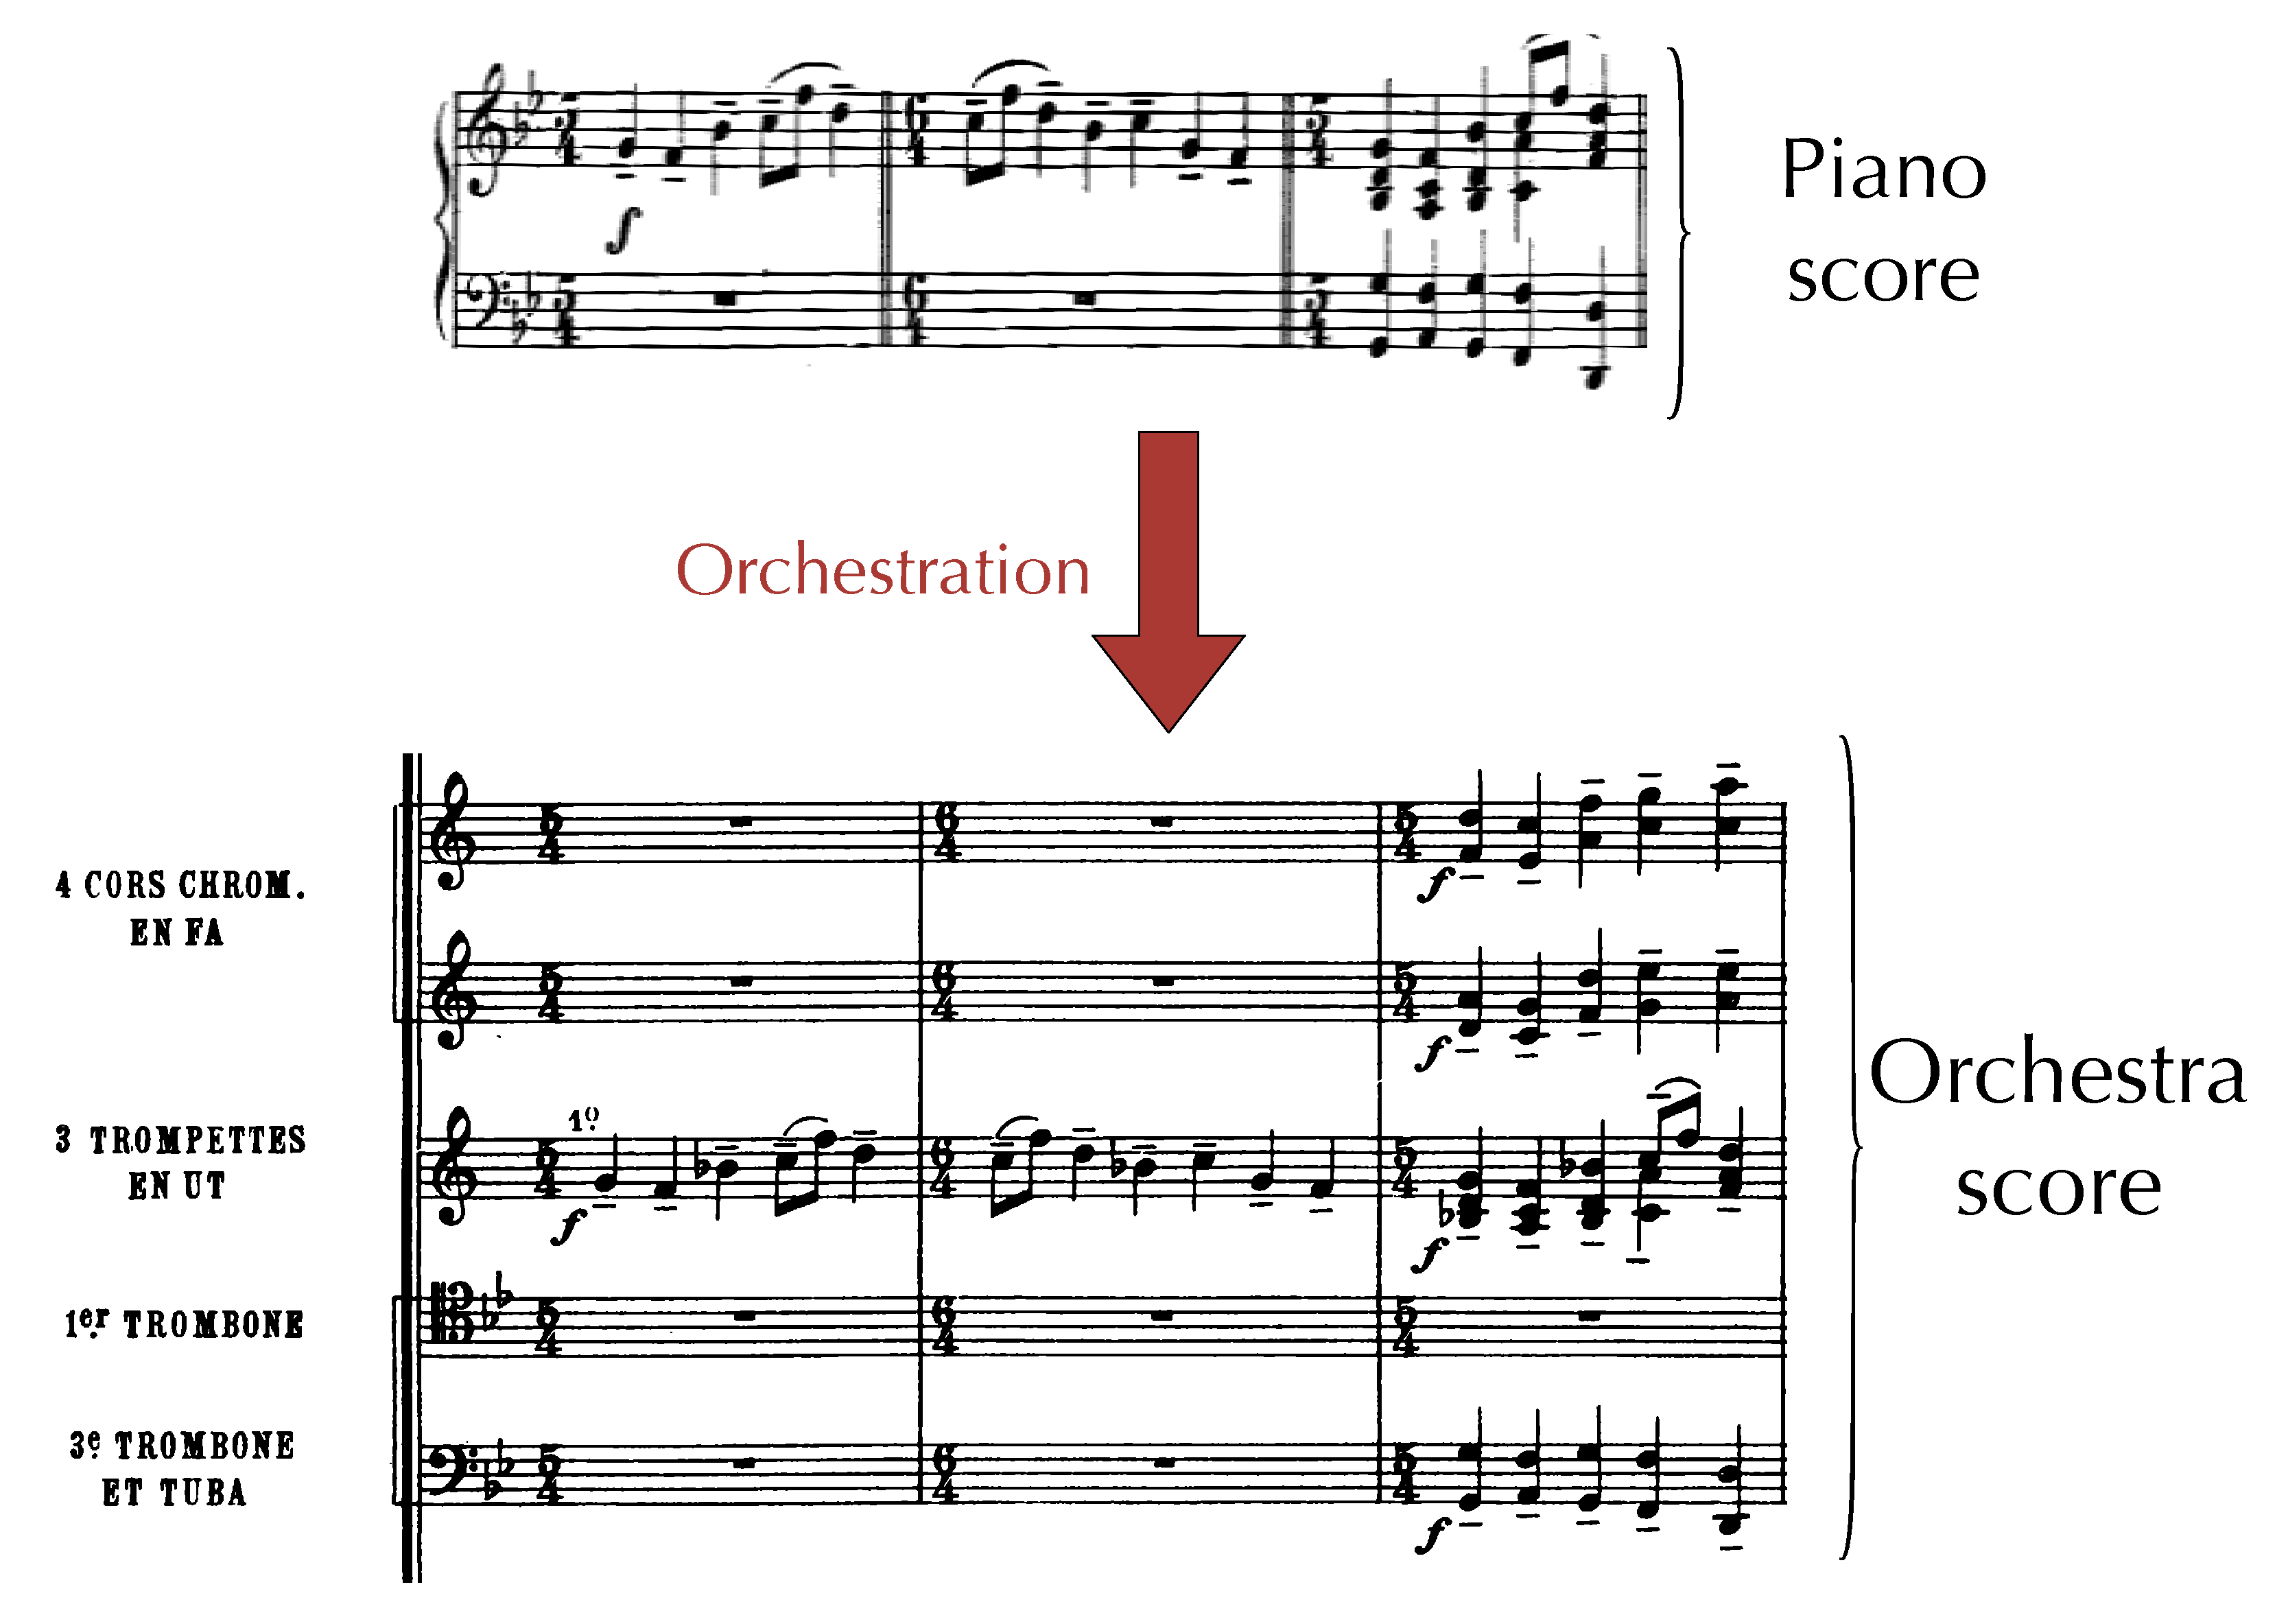
\includegraphics[scale=0.14]{Data_representation/orch}
\caption{\textit{Projective orchestration}. A piano score is projected on an orchestra. Even though a wide range of orchestrations exist for a given piano score, all of them will share strong relations with the original piano score. One given orchestration implicitly embeds the knowledge of the composer about timbre and orchestration.}
\label{fig:orch}
\end{figure}

\subsection{Structure of the database}
\paragraph{Organization}
% Number of file, main aspect a+ Format midi
The Projective Orchestral Database (\textbf{POD}) contains corresponding piano and orchestra scores in the MIDI format.
% Organization, hierarchy
Those files are grouped by pair where the piano score and orchestral version correspond.
Each pair is stored in a folder indexed by a number.
% Where does it come from
The files have been manually collected on several free-access databases \cite{imslp} or entered by professional orchestration teachers \textbf{ON PEUT PEUT-ÊTRE PAS CITER BOULIANE LÀ NON ?}.

\paragraph{Instrumentation}
% CSV instrumentation
As the files gathered in the database have various origins, any given instrument name can be found under a variety of aliases and abbreviations. 
Usually, in the \textit{MIDI} format, each instrument of an orchestral score is represented by a midi track.
Hence, a comma separated value (\textit{CSV}) file is associated to each \textit{MIDI} file with an identical name that links the name of the midi tracks to normalized names of instrument.

\paragraph{Metadata}
% Metadata
At the root of the database folder, a \textit{metadata.csv} file gathers, for each folder, the relative path to the folder from the database root directory, the composer name and the song name for the orchestral and piano works.
% Other statistics
General statistics about the whole database can be found in the \textit{statistics.csv} file such as the number of composers and number of instruments which are reported in \prettyref{tab:stats} \textbf{MEGA USELSESS ca ?}.
\begin{figure}
\centering
\begin{tabular}{lll}
   Number of files & Composers & Instruments\\
   \hline
    &  & 
   \\
\end{tabular}
\caption{BLABLABLA}
\label{tab:stats}
\end{figure}

\paragraph{Integrity}
% Manually checked
Both the metadata and instrumentation \textit{CSV} files have been automatically generated, and then manually checked. We followed a conservative approach when sorting the files. Hence, we automatically rejected any pairs with the slightest ambiguity between a midi track name and a possible instrument (for instance \textit{bass} can refer to \textit{double-bass} or \textit{voice bass}).

\paragraph{Score alignement}
% Aligned and non-aligned versions
Two versions of the database are provided. The first version contains unmodified midi files. The second version contains \textit{MIDI} files automatically aligned using the \textit{Needleman-Wunsch} \cite{NEEDLEMAN1970443} algorithm as detailed in the next section (\prettyref{:automatic-alignment}).

\paragraph{Formats}
% Matrices
We provide several different formats to fasten the research work, such as a piano-roll representation displayed in the \prettyref{fig:piano-roll}. In this case, all the \textit{MIDI} files of piano (respectively orchestra) work have been transformed and concatenated into a unique two dimensional matrix. The starting and ending time of each track is indicated in the \textit{metadata.csv} file.
\textbf{?? Quels formats ??}

\subsection{Automatic alignment}
% Automatic search for projective orchestration match
%\paragraph{Automatic search for pairs}
%A humongous number of \textit{MIDI} files can be found online.
%Although it seems that a lot of piano and orchestra pairs could be uncovered amongst these databases,
%finding them is a tedious task. Indeed, neither their organisation nor their metadata have been thought for the purpose of linking orchestral versions.
%Hence, we tried to form pairs by finding similar file names and music keys, and used the instrumentation to ensure that we have on one side a score for solo instrument, and an orchestral on the other side. 
%For matching file names, a specific fuzzy string matching algorithm based on the \textit{Levenshtein} distance (\cite{fuzzywuzzy}).

% Automatic alignment
% Constat : toutes les partitions ne sont pas alignées
\label{:automatic-alignment}
Given the diverse origins of the \textit{MIDI} files, it is very rare that a piano score and its proposed orchestration are aligned. Indeed, one file can be shorter than the other one, because of temporal dilation factors or skipped parts.
% A quoi ça sert d'avoir des partitions alignées ?
Those misalignments are very problematic for the task that  we introduce in the next section, and in general for any processing which intends to take advantage of the joint information provided between the piano and orchestra scores. Hence, we developed an algorithm to automatically align two scores.
% C'est quoi aligner ? C'est aligner les séquences d'accords formées par le piano-roll
More precisely, we consider the piano-roll representations (\prettyref{fig:piano-roll}) where the scores is represented as a sequence of vectors. Then, we need to define a distance between chords so that the problem of aligning two scores can be casted as a classic sequence alignment problem.
% Definition piano-roll

\begin{figure}[ht]
\centering
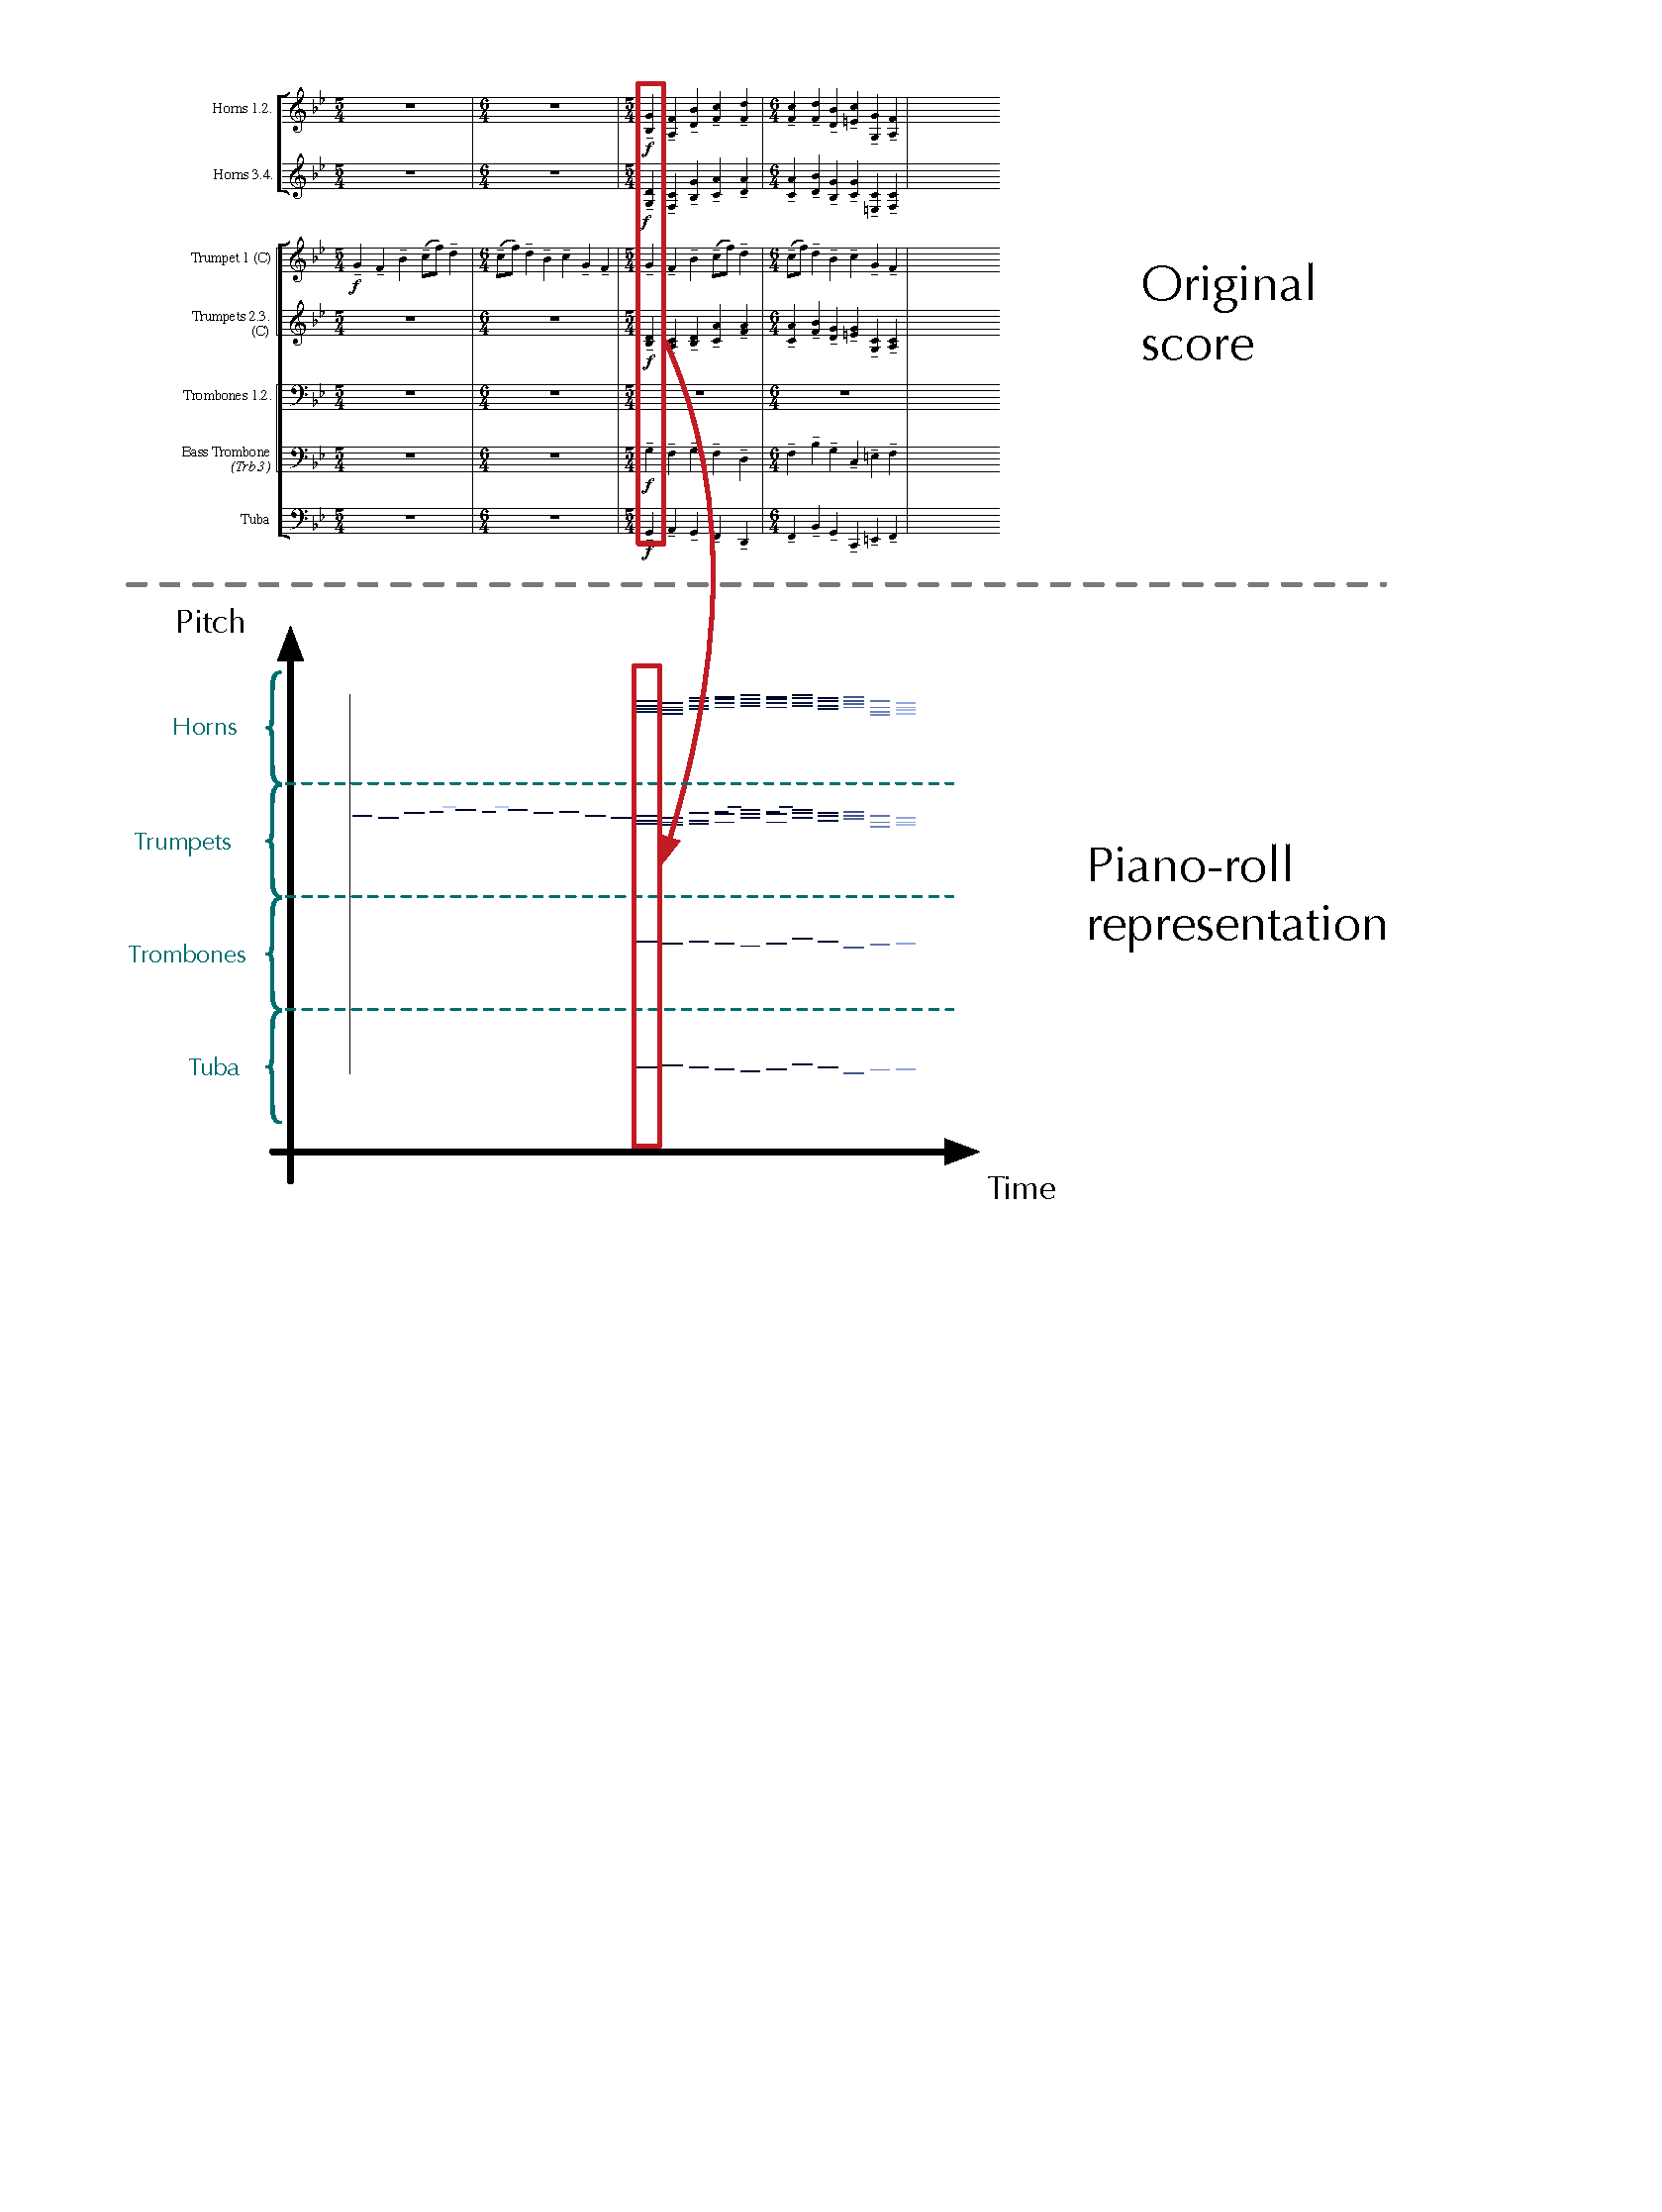
\includegraphics[scale=0.40]{Data_representation/from_score_to_pianoroll}
\caption{A convenient representation of an orchestral score for computer processing is the \textit{piano-roll}. A piano-roll $pr$ is a matrix whose rows represent pitches and columns represent a time frame depending on the discretization of time. A pitch $p$ at time $t$ played with an intensity $i$ is represented by $pr(p,t) = i$, where $0$ is a note off. This definition is extended to an orchestra by simply concatenating the \textit{piano-rolls} of every instruments along the pitch dimension.}
\label{fig:piano-roll}
\end{figure}

% Aligner une séquence : on sait faire = Needleman
% Description Needleman-Wunsch = align with gaps
\paragraph{Needleman-Wunsch}
The \textit{Needleman-Wunsch} (\textit{NW}) algorithm \cite{NEEDLEMAN1970443} is a dynamic programming technique, which allows to find the optimal alignment between two symbolic sequences by allowing the introduction of gaps (empty spaces) in the sequences.
The only requirement of this algorithm is to define a scoring system through a similarity function and a gap penalty. In our case, defining a similarity function boils down to building a similarity measure between two vectors of a piano-roll.

% Similarity matrix
\paragraph{Similarity function}
To measure the similarity between two chords, we propose the following process :
\begin{itemize}
\item discard intensities by represents notes being played as one and zero otherwise.
\item compute the pitch-class representation of the two vectors which flatten all notes to a single octave vector (12 notes).
In our case, we set the pitch-class to one if at least one note of the class is played.
For instance, we set the pitch-class of C to one if there is one note with pitch C played in the chord.
It can be seen as an extremely rough approximation of the harmony, however as we want to align the overall structure of the pieces this is sufficient for our purposes.
After this step, two vectors of size 12 are obtained.
\item if one of the vectors is only filled with zero, it represents a silence, and the similarity is automatically set to zero (note that the score can be negative).
\item for two pitch-class vectors A and B, we define the score as 
\begin{equation}
S \ = \ 5 \ \times \ \frac{\sum_{i=1}^{12} \delta(A_i , B_i)}{0.5 \ max(||A+B||_1 , 1)}
\label{eq:score_function}
\end{equation}
with
\[\delta(x) =
    \begin{cases*}
      0 & if x = 0\\
      -1 & if x = 1\\
      1 & if x = 2
    \end{cases*} 
\]




Z
ZZZZZZZZZZZZZZZZZZZZZZZZZZZ
ZZZZZZZZZZZZZZZZZZZZZZZZZZZ
ZZZZZZZZZZZZZZZZZZZZZZZZZZZ
ZZZZZZZZZZZZZZZZZZZZZZZZZZZ
ZZZZZZZZZZZZZZZZZZZZZZZZZZZZZZZZZZZZZZZZZZZZZZZZZZZZZ

Note that the scaling factor 5 in the equation \prettyref{eq:score_function} has been set empirically. However, modifying its value can be compensated by the tuning parameters of the algorithm introduced in the next section.
\end{itemize}


\paragraph{Tuning the algorithm}
% Parametersesling
In addition to defining a score function, the \textit{Needleman-Wunsch} algorithm has to be carefully tuned by two parameters
\begin{itemize}
\item the gap open penalty defines the cost of introducing a gap in one of the two sequence
\item the gap extend penalty defines the cost of extending a gap in one of the two sequence
\end{itemize}
% Determining the parameters : grid-search
\textbf{The value of those parameters have been set by running a grid-search. Instead of the cumulative scores of the two aligned sequences, which depends on the value of the gap open and gap extend parameters, we used the number of}

Z
ZZZZZZZZZZZZZZZZZZZZZZZZZZZ
ZZZZZZZZZZZZZZZZZZZZZZZZZZZ
ZZZZZZZZZZZZZZZZZZZZZZZZZZZ
ZZZZZZZZZZZZZZZZZZZZZZZZZZZ
ZZZZZZZZZZZZZZZZZZZZZZZZZZZZZZZZZZZZZZZZZZZZZZZZZZZZZ
\section{Case study : projective automatic orchestration}

In this section, we introduce and formalize the automatic projective orchestration task (\prettyref{fig:orch}). In particular, we propose a system based on statistical learning and define an evaluation framework based on the \textbf{POD} database.

\subsection{Task definition}
\paragraph{Orchestral inference}
For each orchestral piece, we define $O$ and $P$ as the sequences of column vectors from the \textit{piano-roll} of the orchestra and piano parts, with $t \in \left[ 1,N_{T} \right]$ where $N_{T}$ is the length of the musical piece, given a particular quantization.

The objective is to design a function that is able to infer the present orchestral frame knowing the recent past of the orchestra sequence and both the past and present of the piano sequence. Mathematically, it consists in designing a function $f$ where
\begin{equation}
\begin{aligned}
\hat{O}(t) = \bm{f}\lbrack & O(t-1), ..., O(t-N), & \\
	& P(t), ... ,P(t-N) \rbrack & \forall t \in \left\lbrack|1, ... N_{T}|\right\rbrack\\
\end{aligned}
\label{eq:inference_function}
\end{equation}
$N$ defines the order of the model. A model with a larger order is expected to perform better.

\paragraph{Evaluation framework}
We propose an \textit{event-level orchestral inference} task to compare the performances of different models.
% Méthode générale
The proposed evaluation consists in splitting the database between a \textit{train} and a \textit{test} subsets. Note that those two subsets must be carefully kept disjoint \cite{bishop2006pattern}. Then, for each file of the test subset and for a given time index $t > N$, where N is the order of the model, the output $\hat{O}(t)$ given by \prettyref{eq:inference_function} can be compared to the ground-truth $O(t)$ from the file.

% Event level
Traditionally, in the music generation field, the comparison between the ground-truth and the model output is made for each time frame \cite{DBLP:journals/corr/YaoCVDD15,boulanger2012modeling,lavrenko2003polyphonic}. However, we have discovered that a model which simply repeats the previous frame gradually becomes the best model as the quantization gets finer. Actually, this we have already observed this phenomenon for a quantization as coarse as four.
Hence, we introduce an event-level evaluation framework where the comparisons between the ground-truth and the model output is only performed for time indexes in $T_e$ defined as the set of indexes $t_{e}$ such that
\[\text{O}(t_{e}) \neq \text{O}(t_{e} - 1)\]

% Comment comparer deux instants
To compare the inferred and ground-truth frames at a time index $t \in T_e$, the accuracy measure commonly used in the music generation field \cite{DBLP:journals/corr/YaoCVDD15,boulanger2012modeling,lavrenko2003polyphonic} is defined as
\begin{equation}
\text{Accuracy}(t)  = \frac{TP(t)}{TP(t) + FP(t) + FN(t)}
\label{eq:accuracy}
\end{equation}
where $TP(t)$ (true positives) is the number of notes correctly predicted (note played in both $\hat{O}(t)$ and $O(t)$). $FP(t)$ (false positive) is the number of notes predicted which are not in the original sequence (note played in $\hat{O}(t)$ but not in $O(t)$). $FN(t)$ (false negative) is the number of unreported notes (note absent in $\hat{O}(t)$, but played in $O(t)$).

% Au final, on mean simplement les différents score obtenus sur chaque event
Finally, the mean accuracy measure over the dataset is given by
\begin{equation}
\frac{1}{K} \sum_{s \in \mathcal{D}_{test}} \sum_{t_e \in T_e(s)} Accuracy(t_e)
\end{equation}
where $\mathcal{D}_{test}$ define the test subset, $T_{e}(s)$ the set of event time indexes for a given score s, and $K = \sum_{s \in \mathcal{D}_{test}} |T_e(s)|$

\subsection{Proposed model}
We proposed a learning based approach, and developed N models. Their detailed description can be found in this article \textbf{REFFERRENEDCOSIDJPSDOC}.
The models we explored are defined in a probabilistic framework, were the vectors $O(t)$ and $P(t)$ are represented as random variables. The orchestral inference function takes the form of a neural network which expresses the conditional dependencies between the different variables (past, and present, orchestra and piano). The likelihood is used as a training objective.

\paragraph{Data representation}
In order to process the scores, we import them as \textit{piano-roll} matrices (see \prettyref{fig:piano-roll}). 
Its extension to orchestral scores is obtained by concatenating the \textit{piano-rolls} of each instrument along the pitch dimension.

%train que sur les event level
For the scores from the training set, only the new events $t_e \in T_e$ are written in the piano-roll.
%approximation = rythmic structure du piano -> rhythmic strucutre de l'orchestre
Hence, the trained model apprehend the scores as a succession of events with no rhythmic structure.
This is a simplification which consists in considering that the rhythmic structure of the projected orchestral score is exactly the same as the one of the original piano score. 
This is false in the general case, since a composer can decide to add nonexistent event in an orchestration.
\textbf{BUT REASONNABLE APPROX}
During the generation of an orchestral score given a piano score, the next orchestral frame is predicted in the event level framework, but injected at the temporal location of the corresponding piano frame \prettyref{fig:event_level_generation}.

\begin{figure}
\centering
\includegraphics{}
\caption{heading}
\label{fig:event_level_generation}
\end{figure}

In order to reduce the input dimensionality, we systematically remove, for each instrument, any pitch which is never played in the training database. Hence, the dimension of the orchestral vector decreased from 2432 to 456 and the piano vector dimension from 128 to 88.
Also, we follow the usual orchestral simplifications used when writing orchestral scores by grouping together all the instruments of the same section. For instance, the \textit{violin} section, which might be composed by several instrumentalists, is written as a single part.
Finally, the velocity information is discarded, since we use binary units which solely indicate if a note is on or off.

\paragraph{Results}
Four models are evaluated on the orchestral inference task. The first model is a random generation of the orchestral frames from a Bernoulli distribution of parameter $0.5$. The second model predicts an orchestral frame at time $t$ by repeating the frame at time $t-1$. Those two naive models constitute a first baseline against which we compare the cRBM and FGcRBM models.

The results are summed up in \prettyref{tab:result_event_level}. As expected, the random model has poor results. The repeat model performs significantly better. Indeed, it is relatively common that a note is sustained between two successive events. The cRBM largely outperforms those two models. However, the FGcRBM model has a lower score than the repeat model. We observed that the activation function of the visible units during the generative step was extremely noisy, which suggests that the training procedure mostly failed. We believe that this is due to the number of parameter,  and especially the dimension of the feature units. Indeed, in \cite{taylor2009factored}, only ten different configuration of the feature units were possible. When training on an orchestral database,  each different piano frame define a different configuration.

\begin{table}[h]
\centering
\begin{tabular}{c c}
\hline
Model & Orchestral Event-level (\%)\\
\hline
Random & 0.5\\ 
Repeat & 12.6\\
\hline \hline
cRBM & 23.2\\ 
FGcRBM & 6.2\\ 
\end{tabular}
\caption{Event-level accuracy for the orchestral inference task. Even though the cRBM performances increase by a factor 3 between the cRBM and the random model, the inclusion of features units provides a leap in the accuracy by multiplying the performances by 4.}
\label{tab:result_event_level}
\end{table}

\subsection{Limits of this framework}
% Limits of this task
% Ground-truth is not only truth

\section{Conclusion and future works}

\bibliographystyle{plain}
\bibliography{../Biblio/biblio}

%----------------------------------------------------------------------------------------

\end{document}
